\documentclass[12pt]{article}
\usepackage[utf8]{inputenc}
\usepackage[T1]{fontenc}
\usepackage[english]{babel}
\usepackage{ifpdf}
\usepackage{newtxtext}
\usepackage{newtxmath} 
\usepackage{array}
\usepackage{graphicx}
\graphicspath{ {./} }
\usepackage{dcolumn}
\usepackage{multirow}
\usepackage{hevea}
\usepackage{abstract}
\usepackage{hanging}
\usepackage{fancyhdr}
\usepackage{float}
% change next 3 lines each issue
\newcommand{\jhead}{Group Project Report - The Anomalies}
\topmargin=-.3in \oddsidemargin=.3in \evensidemargin=.3in \textheight=9in \textwidth=6in
\pagestyle{fancy} 
\fancyhead[L]{\protect\small \href{\jref}{\jhead}\jdate}
\fancyhead[R]{\protect\small  Advanced Network Management 2020\textbf{}} % replace with running head
\fancypagestyle{first-page}{%
 \lhead{\protect\small \href{\jref}{\jhead}}
 \rhead{}
}
\usepackage[labelfont=sc,textfont=sf]{caption}
\usepackage[hyperfootnotes=false,breaklinks=true]{hyperref}
\urlstyle{rm}
\usepackage[hyphenbreaks]{breakurl}
\usepackage{booktabs}
\newcolumntype{L}[1]{>{\raggedright\arraybackslash }p{#1}}
\newcolumntype{C}[1]{>{\centering\arraybackslash }p{#1}}
\newcolumntype{R}[1]{>{\raggedleft\arraybackslash }p{#1}}
\newcolumntype{d}[1]{D{.}{.}{#1}}
\newcommand{\mc}{\multicolumn}
\setlength\tabcolsep{1mm}
\setlength\columnsep{5mm}
\setlength\abovecaptionskip{1ex}
\setlength\belowcaptionskip{.5ex}
\setlength\belowbottomsep{.3ex}
\setlength\lightrulewidth{.04em}
\renewcommand\arraystretch{1.2}
\renewcommand{\topfraction}{1}
\renewcommand{\textfraction}{0}
\renewcommand{\floatpagefraction}{.9}
\widowpenalty=1000
\clubpenalty=1000
\setlength{\parskip}{0ex}
\let\tempone\itemize
\let\temptwo\enditemize
\let\tempthree\enumerate
\let\tempfour\endenumerate
\renewenvironment{itemize}{\tempone\setlength{\itemsep}{0pt}}{\temptwo}
\renewenvironment{enumerate}{\tempthree\setlength{\itemsep}{0pt}}{\tempfour}

\setcounter{page}{1} 

\title{Micro-Service System Troubleshooting}

\author{
Henry Zheng\hspace{0.6cm} Sahand Sabour\hspace{0.6cm}  Samuel Pegg\\
2020280596 \hspace{0.95cm}2020280401  \hspace{0.95cm}2020280261\\
 \{zheng-jh20, shanm20, peggsr10\}@mails.tsinghua.edu.cn
}

\date{} % leave empty
\begin{document}

\begin{htmlonly}
\href{\jref}{\jhead}, \jdate, pp.\
\end{htmlonly}

\maketitle
\thispagestyle{first-page}

\begin{abstract}
\noindent With the rapid growth of large micro-service based systems, detecting anomalies in system operations has become a significantly essential task. In addition, the root causes of such anomalies must also be detected to prevent major costs and losses. Due to the large number of existing calls and complex relationships between different micro-services in modern systems, manual inspection of such micro-services has become extremely challenging and rather impossible. Hence, developing a set of methods that accomplish these tasks within a timely manner and with high accuracy is highly necessary. In this report, we propose an online algorithm that analyzes data generated from a micro-service based system and detects the occurring anomalies and their corresponding root causes.  

\smallskip
\noindent
\textbf{Keywords:} micro-service, anomaly detection, root cause analysis and detection
\end{abstract}


\section{Introduction}
With the recent trends, increasing number of modern day large-scale systems are utilizing micro-services in their system architecture design. In a micro-service based architecture, the system operations are provided as different services, which are loosely coupled (i.e. independent from each other), organized, and highly maintainable, analyzable, and testable. Hence, this type of architecture allows large-scale and complex systems to provide faster and more reliable services to their users. However, a major disadvantage of these systems is the massive number of calls between different services and their complex relationships; which in turn makes finding faulty services and errors rather challenging.

\noindent In the case that a faulty micro-service causes an error in the system, this occurrence would be referred to as an anomaly, which should be detected as soon as possible. Accordingly, the anomaly should be traced back to the faulty service that caused it. This process is referred to as troubleshooting and by accomplishing this task, the system maintainers would be able to fix the faulty service and any subsequent problems before experiencing major costs and losses. Therefore, implementing an algorithm that detects system's anomalous behavior and is able to both accurately and efficiently identify its root cause is essential.

\noindent In this project, we were tasked to design an online algorithm to perform these tasks on an incrementally published dataset (i.e. real-time data) generated by a micro-service based system through Kafka producer. More specifically, our task was to analyze the provided time series data, detect anomalous behavior, discover anomalous system nodes at the time of this occurrence, and find the Key Performance Indicator (KPI) that is the root cause of this anomaly. The rest of this report is organized as follows: in section 2, we summarize the relative literature for these tasks and acknowledge the work of top teams for this competition; in section 3, we further explain the problem statement and provide our implemented algorithms for this project; section 4 includes a discussion of our results as well as the lessons learned; lastly, we conclude the report in section 5. 

\section{Previously Implemented Work}
As mentioned, micro-service based large-scale systems consists of large number of complex calls and relationships between different services. In addition, once a service in the system becomes unavailable, unstable, and/or impaired, detecting and fixing this system in a timely and accurate manner is the top priority. Due to the large amount of data to be analyzed, manual inspection has proven to be hugely time consuming and overall, an ineffective approach. Hence, considerable research has been conducted to automatically analyze and detect such failures and their causing factors.


\noindent The problem statement for anomaly detection and localization is fairly simple: use historical data or a stream of seasonal data as a time series from a micro-service based system to detect any anomalies and find the root cause. Donut [1] and Bagel [2] managed to accomplish this task by utilizing variational auto-encoders (VAEs). However, even though these models achieved satisfactory results for our task, they also needed sufficient resources for training and processing. Given that we were not provided with any GPUs for this project, we deemed they were not suitable for our project due to the running time. They also do not provide host KPI localisation. The next approach we attempted, TraceAnomaly [3], a deep Bayesian network based algorithm, suffered similar setbacks as it is a deep learning algorithm requiring a GPU. It ran quite slowly, and while it could produce the correct host, it gave us no information towards finding the KPIs. A very attractive solution was MicroRCA [4] as their proposed framework and studied cases strongly resembled this competition. Their approach is illustrated in Figure \ref{fig:RCA Overview}.
\begin{figure}[H]
    \centering
    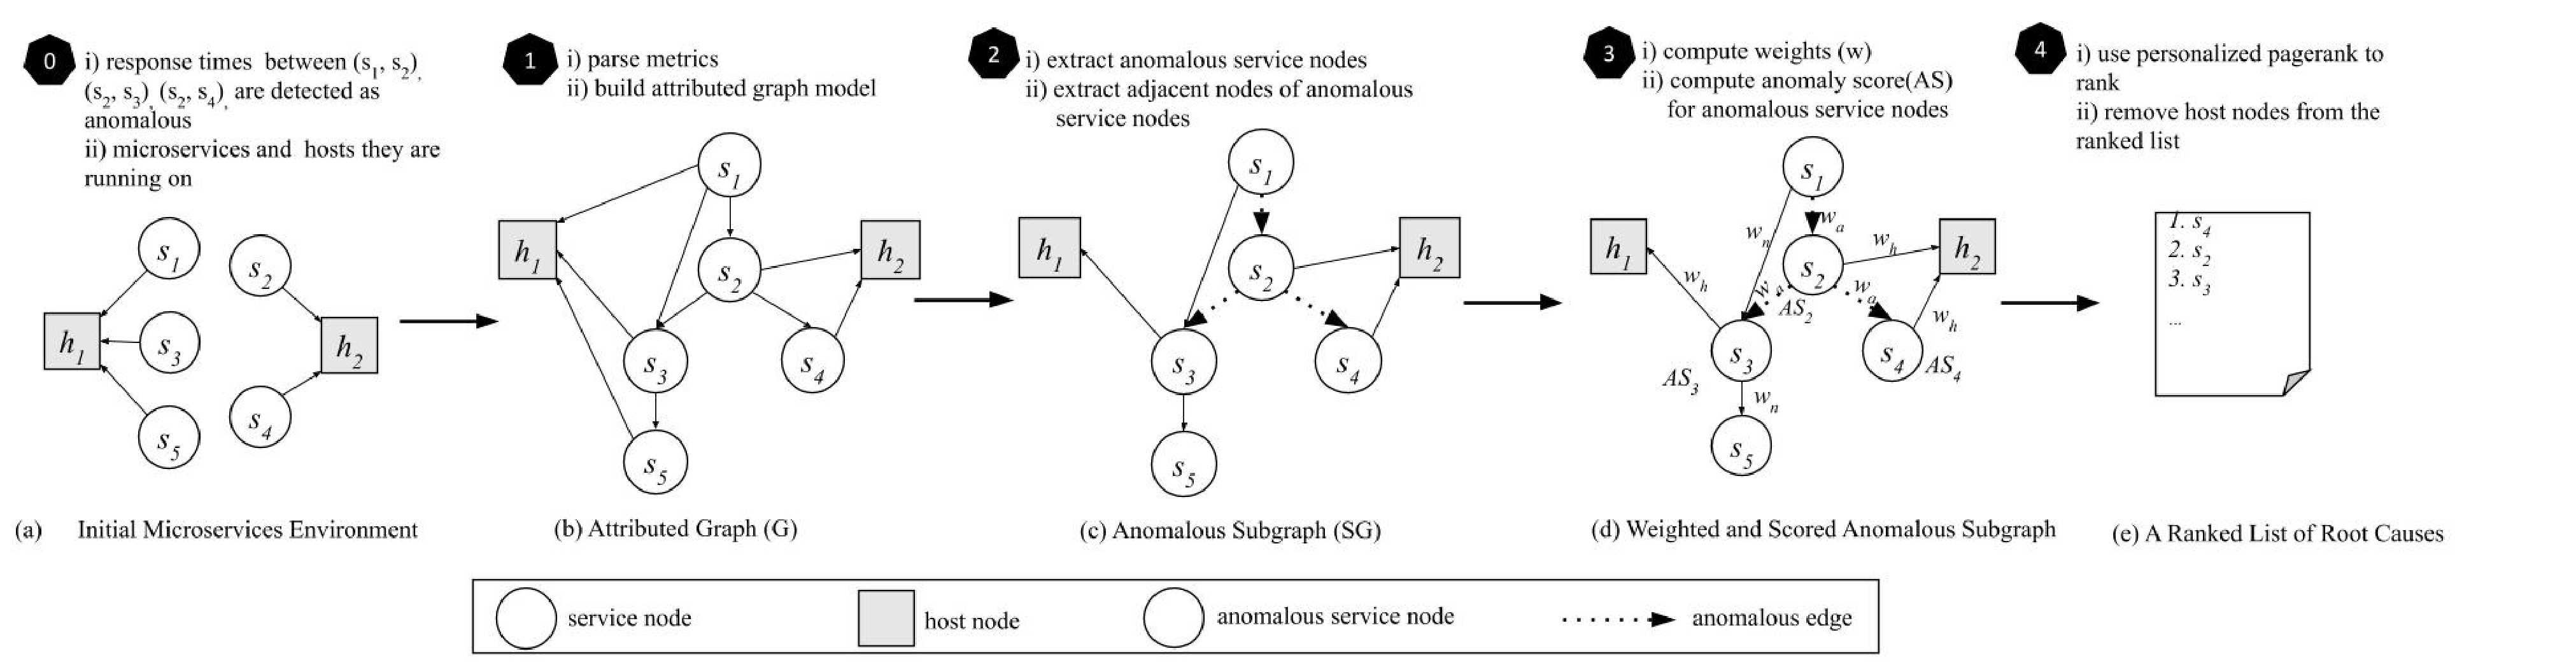
\includegraphics[width = \linewidth]{microRCA.eps}
    \caption{RCA Overview [4]}
    \label{fig:RCA Overview}
\end{figure}

\vspace{-0.3cm}
\noindent MicroRCA utilizes BIRCH [5] to detect the anomalous edges, and uses various formulas to assign weights to the edges of the sub-graph. The nodes themselves are weighted using Pearson correlation between the anomalous edges and the host KPI data. We implemented the original method and tried many different variations in order to get the method to produce a list of hosts and KPIs. However, the Personalized PageRank [6] often did not converge, and when it did, the results were not satisfactory. Every variation we tried had its own problems. So despite how attractive MircroRCA first appeared and how related to this competition it was, we decided to remove it from our project.

\noindent Next, we took huge inspiration from H3C AI Institute's slides and managed to implement a solution that produced a score greater than 0. We then combined this approach with the information provided by the other teams after the first deadline in order to streamline our code, remove bugs and improve performance. Regarding the proposed algorithms for this competition, the winning team [7] cleverly discarded one of the three provided data sources to increase the detection speed. Accordingly, they established a set of rules and manually selected thresholds to detect anomalies and localize root causes. Similarly, the runner up team [8] also discarded the first set of provided KPI sources, focused merely on trace data and formulated this problem as a pattern finding challenge in a constructed anomaly table. Lastly, the team in third place [9] utilized the first set of available data to identify the anomalous points, analyzed the second set to detect failed and delayed calls, find abnormal hosts, and extract the necessary features. One of the honorable mentions in their work was that they used dictionaries instead of pandas to improve the algorithm's speed. These simple tips allowed us to improve our method significantly.

\section{Methodology} 
In this section, we describe the provided dataset and our implemented algorithms.

\vspace{-0.2cm}
\subsection{Data}
In this project, we were provided with three KPI data sources: ESB, Trace, and Host data.

\smallskip\smallskip
\noindent \textbf{ESB business indicator (ESB): }is provided every minute and mainly demonstrates the number of requests for the \textit{osb\_001} service and the overall success rate of these request during each minute. Once an anomaly occurs, assuming at a point t in time, the success rate is expected to be lower than 1. Accordingly, it would be recorded to be used for further analysis in the other two KPI data sources.

\smallskip
\noindent \textbf{Trace: }it is provided for every request and consists of several micro-service calls, referred to as spans. This section of the data demonstrates the start and elapsed time for each span, the databases that were accessed (if any), the trace of the span and its host. Upon finding anomalous time t in the ESB data, the time around t is to be investigated in order to detect anomalous spans (i.e. nodes with unusually long response time) and ultimately, realize faulty service nodes. 

\smallskip
\noindent \textbf{Host: }is provided in the (timestamp, value) format and includes the host service name and the called operation. Upon finding the faulty service nodes, this data can be explored to find anomalous values for a KPI, which would then be flagged as a root cause.

\subsection{Dropping ESB Business Indicator}
\smallskip
\smallskip
\noindent Inspired by MicroRCA [4], we utilized BIRCH [5], which is an online clustering-based outlier detection algorithm, to detect anomalies in the ESB data. In this project, we considered comparatively large values for average time and considerably small success rates as anomalous behavior. Hence, we employed BIRCH separately for these two columns and set the BIRCH threshold (i.e. radius) to 0.5 and 0.1 respectively. 


\noindent The algorithm produced good results for a short while. However, a major disadvantage of this implementation was that when the code was left running on the server, the anomaly detection process started happening when the system is in its normal state. Given enough anomalies, the anomalies actually become the normal state of the system. In order to address this problem, we pretrained two separate BIRCH models for average time and success rate respectively on the provided two weeks of data with all anomalous data removed.


\noindent Upon detecting an anomaly in the ESB data, we would stop analyzing incoming data until a root cause is found. Accordingly, we would send the timestamp of the detected anomaly to the next module for faulty service detection in trace data. The incoming data would not be discarded but rather stored in a separate storage for future analysis.


\noindent However, this approach also proved to be sub-optimal. The reason being, the effects of many anomalies are often quite significantly delayed in the ESB data - indeed, some anomalies do not cause any change in the ESB data. Thus waiting on the ESB data for anomalies was inefficient and sometimes causing us to miss anomalies. Hence we decided to remove this method from our project and fully discard ESB data.


\subsection{Final Solution Design}
\smallskip\smallskip
Figure \ref{fig:overview} illustrates an overview of our method's architecture. At a high level, the proposed framework could be divided into three sections: data collection, anomalous host localization, anomalous KPI localization.
\begin{figure}[H]
    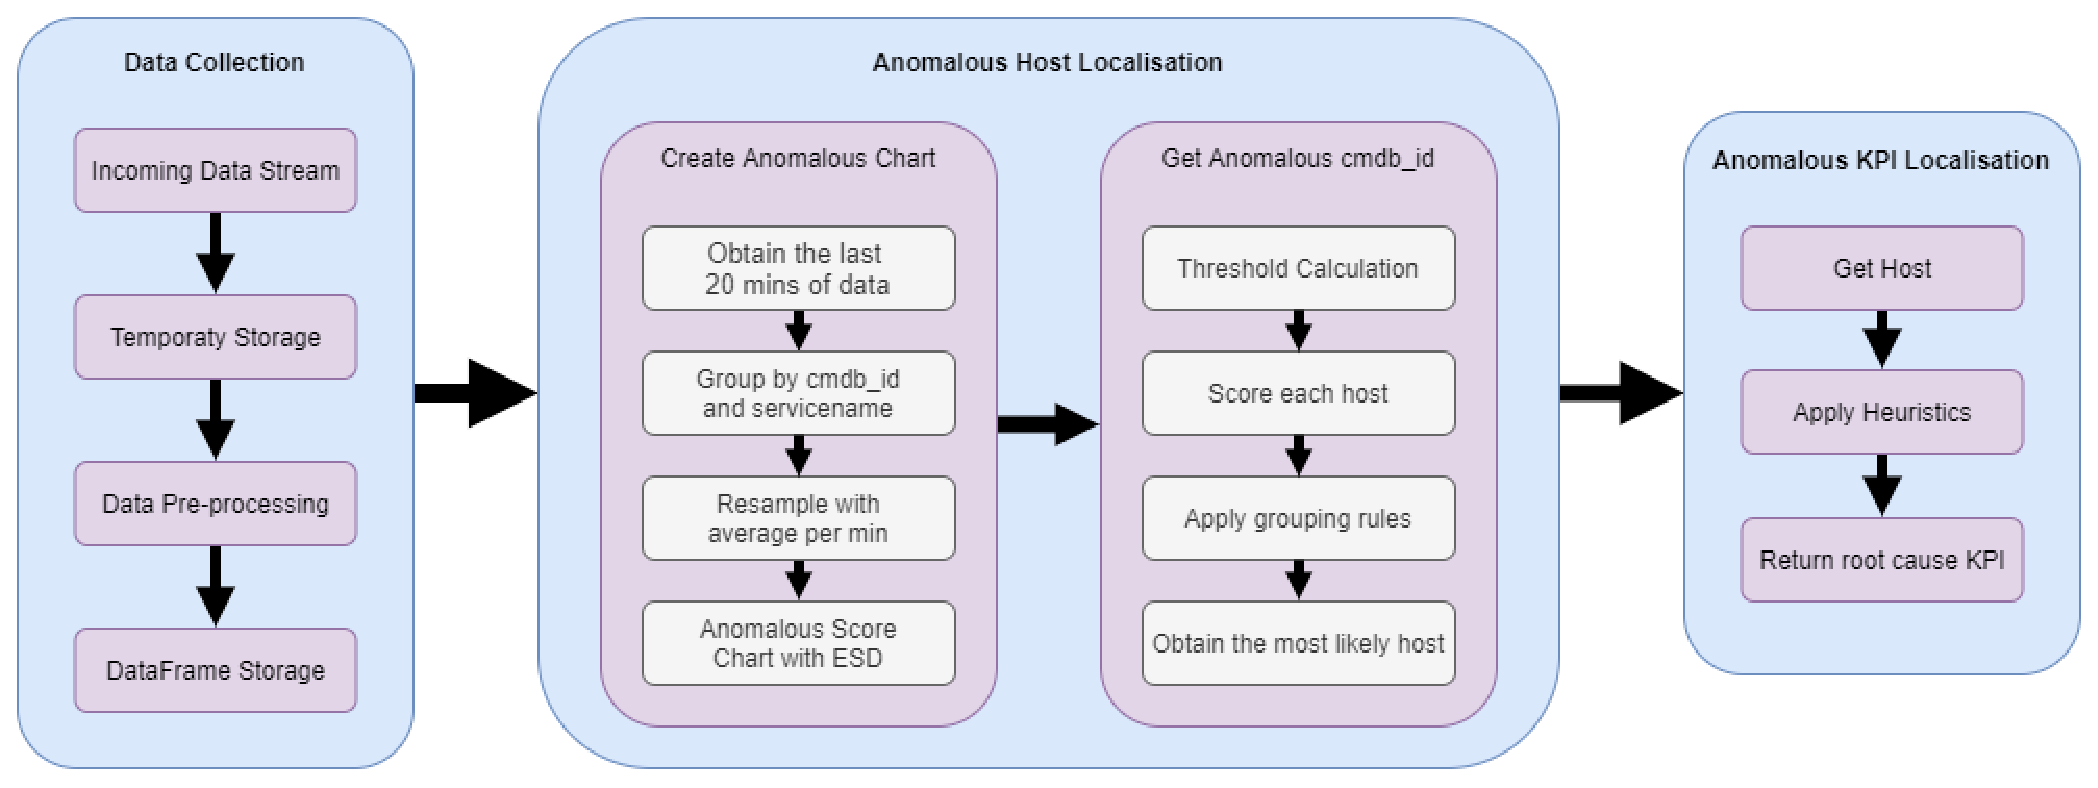
\includegraphics[width=\columnwidth]{ANM Diagram.eps}
    \caption{Proposed method architecture}
    \label{fig:overview}
\end{figure}


\subsubsection{Data Collection}
\textbf{Code Architecture:} The final code architecture in our submission is composed of 2 threads: a main thread and a worker thread. The main thread is responsible for collecting the incoming data from the Kafka server and adding it into temporary storage. It runs for every new item of Kafka data. The worker thread runs periodically every minute. It takes all the data collected by the main thread out of temporary storage and processes and prepares before adding it to the main data storage. It then performs anomaly detection and localization on the main data storage.

\smallskip
\noindent\textbf{Data Retrieval:} This process is handled by the main thread. We have three types of data (ESB, Trace and Host KPI). As previously mentioned, we immediately discard any ESB data, but the trace data and host KPI data are stored in memory via a temporary 1 minute storage dictionary. During this process, we make minor adjustments to the trace data. As the parents of \textit{JDBC} spans are \textit{LOCAL} spans, the trace logs of \textit{LOCAL} types can effectively represent the \textit{JDBC} spans; that is, if the \textit{JDBC} spans are anomalous, it will be shown in the logs of the \textit{LOCAL} spans. Hence, all the \textit{JDBC} trace logs are discarded by our program. Every minute, the worker thread collects the data from the temporary dictionary and adds it to the main DataFrame storage. This data only stays in memory for a total of 20 minutes and is deleted afterwards.

\smallskip
\noindent \textbf{Data Processing:} The worker thread takes care of data processing. We only process the trace data as Host KPI data is already in the desired format, which is done as follows:
\begin{itemize}
    \item If CallType is \textit{OSB} or Remote Process, we replace the ServiceName with cmdb\_id.
    \item If CallType is \textit{CSF}, we replace the serviceName with the cmdb\_id of its child.
    \item If CallType is \textit{LOCAL}, we replace the serviceName with dsName.
    \item For each span, we deducted the total elapsedTime of each of its child spans. 
\end{itemize}
The final step is highly essential as it allows us to determine where the problem is more accurately. This means the processed logs are more independent than the original data. For example, suppose we have a \textit{LOCAL} service acting anomalously. Without this pre-processing step, the anomaly would also be reflected in the \textit{OSB} data, and hence anomaly detection would return an \textit{OSB} anomaly such as \textit{os\_021}. To write this more formally
\[
    \textit{Actual elapsedTime}=  elapsedTime - \sum \textit{elapsedTime of children}
\]
\subsubsection{Host Localization}
For host localization, the processed trace data is used. As mentioned above, we have 20 minutes of processed data stored, which is updated every minute. We group this trace data by ``cmdb\_id`` and ``serviceName`` for anomaly detection. This allows us to group the data by the edges of the graph representing the data topology, seen below. After the processing, cmdb\_id and serviceName effectively stand for `parent cmdb\_id' and `child cmdb\_id' respectively, so each grouping represents a call from the parent cmdb\_id to the child cmdb\_id. All unique possible calls are shown below (Figure \ref{fig:Topology}). Note that each cmdb\_id also has a self loop/edge too, which is not shown.
\begin{figure}[H]
    \centering
    
\includegraphics[width = .8\linewidth]{topology.eps}
    \caption{Data Topology}
    \label{fig:Topology}
\end{figure}
\subsubsection*{3.3.2.1 Host Localization - Anomaly Score Chart}
The figure below shows the next step of our anomaly detection: the anomaly score chart. Compared to our previous unstable/slow implementations, simpler methods were proven better than complex methods. Thus, we decided on using a anomaly score chart for better visualization of anomalies and anomaly detection. A sample Anomaly Chart can be seen in Figure \ref{fig:Anomaly Score Chart}. In this section we discuss how these Anomaly Charts are created.
\begin{figure}[H]
    \centering
    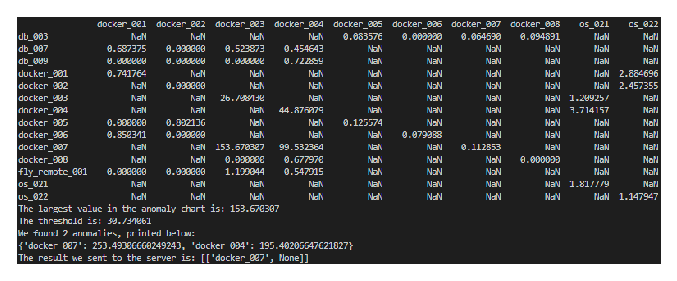
\includegraphics[width = \linewidth]{Score Chart.eps}
    \caption{Anomaly Score Chart}
    \label{fig:Anomaly Score Chart}
\end{figure}
\noindent
\textbf{Anomaly Score Calculation:} For each of the groups, which represent a call path, we calculate the following values: first, we calculate the average elapsedTime of each minute of data in the 20 minutes worth of stored data. This gives us 20 points of data for each call path; Second, the top 10\% anomalous data points for each call path are found using Seasonal Hybrid Extreme Studentized Deviate (S-H-ESD)[10]. To explain S-H-ESD, we introduce the following notation.
\begin{equation}
    R_j = \frac{\max_i |X_i - median(X)|}{MAD}, \quad 1 \leq j \leq k
    \label{eq:esd_test}
\end{equation}

\[
    \text{where }  MAD = median(|X_i - median(X)|)
\]

\begin{equation}
    \lambda_j = \frac{(n-j) * t_{p,n-j-1}}{\sqrt{(n-j-1+t_{p,n-j-1}^2)(n-j+1)}}, \quad 1 \leq j \leq k 
    \label{eq:esd_critical}
\end{equation}
The Residual $R_j$ is found for every data point in a group. Then, the anonymity of each data point in a group is calculated by comparing the Residual $R_j$ with its critical value $\lambda_j$. Any Residuals $R_j$ higher than the critical value $\lambda_j$ is flagged as anomalous. The $Anomaly\ Score$ of the elapsedTime column for each group is computed using the flagged anomalous data points as follows. Let $X$ be the 20 values in a particular grouping. We calculate:
\[
    ESD_{result} = \sum(|X_{anomalous} - median(X)|)
\]

\noindent Since, the database (db) anomalies are not obvious just by looking at the elapsedTime column, we also incorporate a $Failure\ Score$ into our $Anomaly\ Score$. The $Failure\ Score$ is the number of failed calls in the data for each group. The ``success" column of the trace data a Boolean, so we calculate
\[
    Failure\ Score =  \sum success\ column == False
\]

\noindent Note that we only calculate $Failure\ Score$ for groupings where the serviceName (i.e. the child cmdb\_id) is a database. Lastly, the overall $Anomaly\ Score$ for the current cmdb\_id and serviceName pair is computed as follows:
\[
    Anomaly\ Score = ESD_{result} + Failure\ Score
\]

\noindent Once we have computed the $Anomaly\ Score$ for each possible pairing of cmdb\_id and serviceName, we have all the entries to construct the Anomaly Chart, as seen in Figure \ref{fig:Anomaly Score Chart}. 

\subsubsection*{3.3.2.2 Host Localization - Score Chart Analysis}
Looking at Figure \ref{fig:Anomaly Score Chart}, we can see high scores in docker 3, 4 and 7 rows/columns. This section details how we decide which cmdb\_id is anomalous. From the GitHub datasets containing the ground truth, there is only one anomalous cmdb\_id during each anomaly, but simply selecting the row from the table with the largest value often is not sufficient. Hence we perform the following steps to produce a more efficient solution.

\smallskip
\noindent \textbf{Threshold Calculation:} Once we get an Anomaly Score Chart from the previous stage, we first calculate the threshold $t_1$ of the anomaly chart. This is the threshold over which we consider an entry in the table to be anomalous. Let $M$ be the maximum value in the table. We found that 20\% of $M$ was a good indicator for anomalous entries. However, since we run detections every minute, we still create tables even when there are no anomalies present. To deal with this issue, we set a minimum threshold of 10, which was decided after thorough observations of the anomaly chart. Hence, in the case of a normal table, no anomalies would be detected. The threshold calculation is summarized as follows:
\[
    t_1 = \max\left(\frac{M}{5}, 10\right)
\]

\noindent \textbf{cmdb\_id Scores:} For each cmbd\_id, we calculate the mean of the row sum and the column sum (when the column exists). Looking at Figure \ref{fig:Topology}, this mean essentially represents the mean of the sum of the in edges and the sum of the out edges. Let $i$ denote a particular cmdb\_id and let us denote this mean as $m_i$. Then, using the calculated threshold, for each cmbd\_id, we also calculate the number of anomalous entries in its row and the number of anomalous entries in its column. This is essentially counting how many of the in edges/out edges are anomalous in Figure \ref{fig:Topology}. Let $r_i$ be the number of anomalies in the row, and $c_i$ the number of anomalies in the column. We then calculate 
\[
    a_i = \left\lfloor\frac{2r_i + c_i}{2}\right\rfloor
\]

\noindent Since every non-NaN entry in the table represents a call from column cmdb\_id to row cmdb\_id, we assign extra weight to the destination node as this is more likely to be the problem. However, since this is not always the case, we still need to consider the source node. Next, to assign a score $s_i$ to each cmdb\_id, $i$, we simply calculate $s_i = a_i\times m_i$. We then use an additional threshold $t_2$, which is calculated as
\[
    t_2=\max_{i}\left(\frac{s_i}{10},1\right)
\]

\noindent to filter out the cmdb\_ids with low score ($s_i$) and pass the resulting list onto the next stage. If there are no scores $s_i$ greater than 1, we return an empty list and end the localization.

\smallskip
\noindent \textbf{Grouping rules:} From our observations and the Excel file showing the hosts of the various cmdb\_ids, we realized that there are certain rules that are needed to be applied in order to get better performance. The derived rules are as follows:
\begin{itemize}
    \item If os\_021 and os\_022 are anomalous, the problematic cmdb\_id is os\_001.
    \item If we have docker\_00($x$) and docker\_00($x+4$), the problematic cmdb\_id is actually os\_0($16+x$). For example, if docker\_002 and docker\_006 are anomalous, the problematic cmdb\_id is os\_018.
    \item Note that we have a ``fly remote" row in our anomaly chart, but there is no cmdb\_id called fly remote. The cmdb\_id corresponding to an anomalous fly remote is os\_009.
\end{itemize}
\textbf{Find most likely anomalous cmdb\_id:} If none of the grouping rules are met, we simply send the cmdb\_id with the greatest score to the next stage. Else, we send the successful result of one of the grouping rules. This means we prioritise the grouping rules over score, as this gave us the best performance during the first round of final testing stage.


\subsubsection{KPI Localisation}
Given the anomalous cmdb\_id from the previous stage, we use the following observations to determine the root cause KPIs. 
\begin{itemize}
    \item If the cmdb\_id is of type ``os", i.e. an operating system, the KPIs are always Sent\_queue and Received\_queue.
    \item If the cmdb\_id is of type ``docker", the KPI root cause is either Null or container\_cpu\_used.
    \item If the cmdb\_id is of type ``db", i.e. a database, the KPI root causes are either the combination of Sess\_Connect, Proc\_Used\_Pct and Proc\_User\_Used\_Pct, or the combination of On\_Off\_State and tnsping\_result\_time.
\end{itemize}
So if the cmdb\_id is of type ``os" we can instantly send off a result, but docker and database cmdb\_ids require further analysis to decide between the two options. 
\begin{enumerate}
    \item Docker KPI decision: If the docker-docker entry in the anomaly chart (i.e. a call to itself) is anomalous, the problem is container\_cpu\_used. If the self call is not anomalous, then it must be a network issue, in which case the KPI is Null.
    \item Database KPI decision: To decide between the two options we need only look at the On\_Off\_State KPI data. Note, this is the only purpose the KPI data serves in our method. If there are any 0 values in On\_Off\_State, we return On\_Off\_State and tnsping\_result\_time. If the values for On\_Off\_State are all 1, we return Sess\_Connect, Proc\_Used\_Pct and Proc\_User\_Used\_Pct.
\end{enumerate}
Note that we can see bullet point 1 in action in Figure \ref{fig:Anomaly Score Chart}. The docker\_007 to docker\_007 call only has a value of 0.112853 and is hence not anomalous (since the threshold is 30.7). Thus it must be a network error rather than a cpu error, and hence we return $[[docker\_007, Null]]$.


\subsection{Additional Checks}
Since we run anomaly detection every minute, and we take 1 minute averages of the last 20 minutes of data, sometimes an anomaly is not fully expressed in the data at the time we create the Anomaly Chart. This means that if we blindly send off a result as soon as we get a table with an anomaly, we may send the wrong answer. To solve the issue, when we get a result from the table we store it and wait for anomaly detection to run again a minute later. Only if the two answers are equal do we send off the result to the server. Otherwise, we keep running anomaly detection every minute until the last two results agree. From our observations of the code on the server, the first result is usually correct, and the next result is the same, so we can detect anomalies in two minutes. However, sometimes, particularly for docker anomalies, the database values spike slightly above the threshold of 10 before the docker entries in the table become anomalous. Originally we would have submitted a database anomaly, but now we are correctly able to identify the actual root cause - the docker.

In addition, once we detect an anomaly, since we create the tables from 20 minutes of historical data and anomalies can last up to around 10 minutes, we wait 30 minutes after we detect an anomaly before starting detection again. This is so that we don't continuously send of the same answer again and again. Another reason for this wait of 30 minutes can be explained with the following example. Suppose at time $t_0$ we detect docker\_001. Lets say this anomaly lasts 9 minutes until $t_9$. Then suppose at time $t_24$ there is docker\_005 anomaly. Then the 20 minutes of historical data would have both the docker\_005 and docker\_001 anomalies. This would mean our Anomaly Chart analysis would (incorrectly) return os\_017 as the anomaly, rather than docker\_005.

\section{Discussion and Lessons Learned}
In the final test of this competition, we were able to score 70 points and rank $8^{th}$. After finishing this competition and analyzing the proposed algorithms of the top teams, we believe that we learned a number of valuable lessons throughout this experience. Firstly, data pre-processing is one of the most most important steps needed in order to achieve a sound solution and should not be underestimated. With efficient data processing, the important features of the available data can be extracted. Secondly, during this competition we had the opportunity to work with seasonal data and different deep learning algorithms and approaches, which served as a great learning experience. Thirdly, judging by the methods that scored the most points, we learned that over complicating the problem is not a good idea and we should always start with the most basic heuristics approach in order to get some initial results, which can be expanded upon. Finally, the most valuable lesson of all for us was proof reading and triple checking our code to always make sure that all parts of the program are working as expected. For instance, in the final days of testing the submit function was commented out, which resulted in our team scoring 0 points regardless of our improvements in the code. Hence, to conclude, the overall lesson would be to never take parts of your work for granted and ensure all parts are working as planned, try the simple approaches first, and learn as you work. 
\section{Conclusion}
In conclusion, we proposed a rather robust online algorithm for anomaly detection and root cause localization in micro-service based systems. We tried many different approaches based on our research, the surrounding literature and the proposed methods of fellow competitors. In addition, we demonstrated our proposed methodology and discussed the lessons learned throughout this project. Regardless of the final results, we regard this competition as a valuable learning experience and are proud of our team's hard work to obtain these results. 

\section*{References}
\begin{hangparas}{1em}{1}
[1] Haowen Xu,  Wenxiao  Chen, Nengwen Zhao,  Zeyan  Li, Jiahao  Bu, Zhihan  Li,  Ying Liu,  Youjian Zhao,Dan  Pei, Yang Feng. "Unsupervised Anomaly Detection via Variational Auto-Encoder for Seasonal KPIs in Web Applications". Proceedings of the 2018 World Wide Web Conference on World Wide Web, 2018, pp. 187-196.

\smallskip\smallskip
[2] Zeyan Li, Wenxiao Chen, Dan Pei. "Robust and Unsupervised KPI Anomaly Detection Based on Conditional Variational Autoencoder". 2018 IEEE 37th International Performance Computing and Communications Conference (IPCCC). IEEE, 2018.

\smallskip\smallskip
[3] Ping Liu, Haowen Xu, Qianyu Ouyang, Rui Jiao, Zhekang Chen, Shenglin Zhang, Jiahai Yang, Linlin Mo, Jice Zeng, Wenman Xue, Dan Pei. "Unsupervised Detection of Microservice Trace Anomalies through Service-Level Deep Bayesian Networks". 31th International Symposium on Software Reliability Engineering (ISSRE). IEEE, 2020.


[4] Li Wu, Johan Tordsson, Erik Elmroth, Odej Kao. "MicroRCA: Root Cause Localization of Performance Issues in Microservices". IEEE/IFIP Network Operations and Management Symposium (NOMS), 2020. 

\smallskip\smallskip
[5] A. Gulenko, F. Schmidt, A. Acker, M. Wallschlager, O. Kao, and F. Liu, “Detecting anomalous behavior of black-box services modeled with distance-based online clustering”, in 2018 IEEE 11th International Conference on Cloud Computing (CLOUD), 2018.

\smallskip\smallskip
[6] G. Jeh and J. Widom, “Scaling personalized web search”, in WWW-2003, pp. 271–279.

\smallskip\smallskip
[7] Yunfeng Zhao, Xuanrun Wang, Guojie Fan. "Advanced network management - the Old Driver on Xuetang Road", 2020. 

\smallskip\smallskip
[8] Yixiong Ji, Yunpeng Liu. "Anomaly Detection and Root Cause Localization in Microservice System - meow meow group", 2020.

\smallskip\smallskip
[9] Zhangzi Hao, Yaoyu Zhang, Shaohuai Liu. "ANM project - Veritaserum", 2020. 

\smallskip\smallskip\noindent
[10] Jordan Hochenbaum and Owen S. Vallis and Arun Kejariwal. "Automatic Anomaly Detection in the Cloud Via Statistical Learning"

\vfill % use this for column breaks
\break

\end{hangparas}

\end{document}
